\section{The Nyaya Reasoning Framework}
\label{sec:nyaya}

Navya-Nyaya (``New Logic'') represents a sophisticated epistemological system developed in medieval India that integrates logical reasoning with epistemic validation. Unlike Western formal logic, which focuses primarily on syntactic validity, Nyaya emphasizes the epistemic sources of knowledge and requires explicit grounding of abstract reasoning in concrete examples (\textit{dṛṣṭānta}). This section presents our computational adaptation of the six-phase Nyaya methodology, detailing both theoretical foundations and practical implementation requirements.

\begin{figure}[t]
\centering
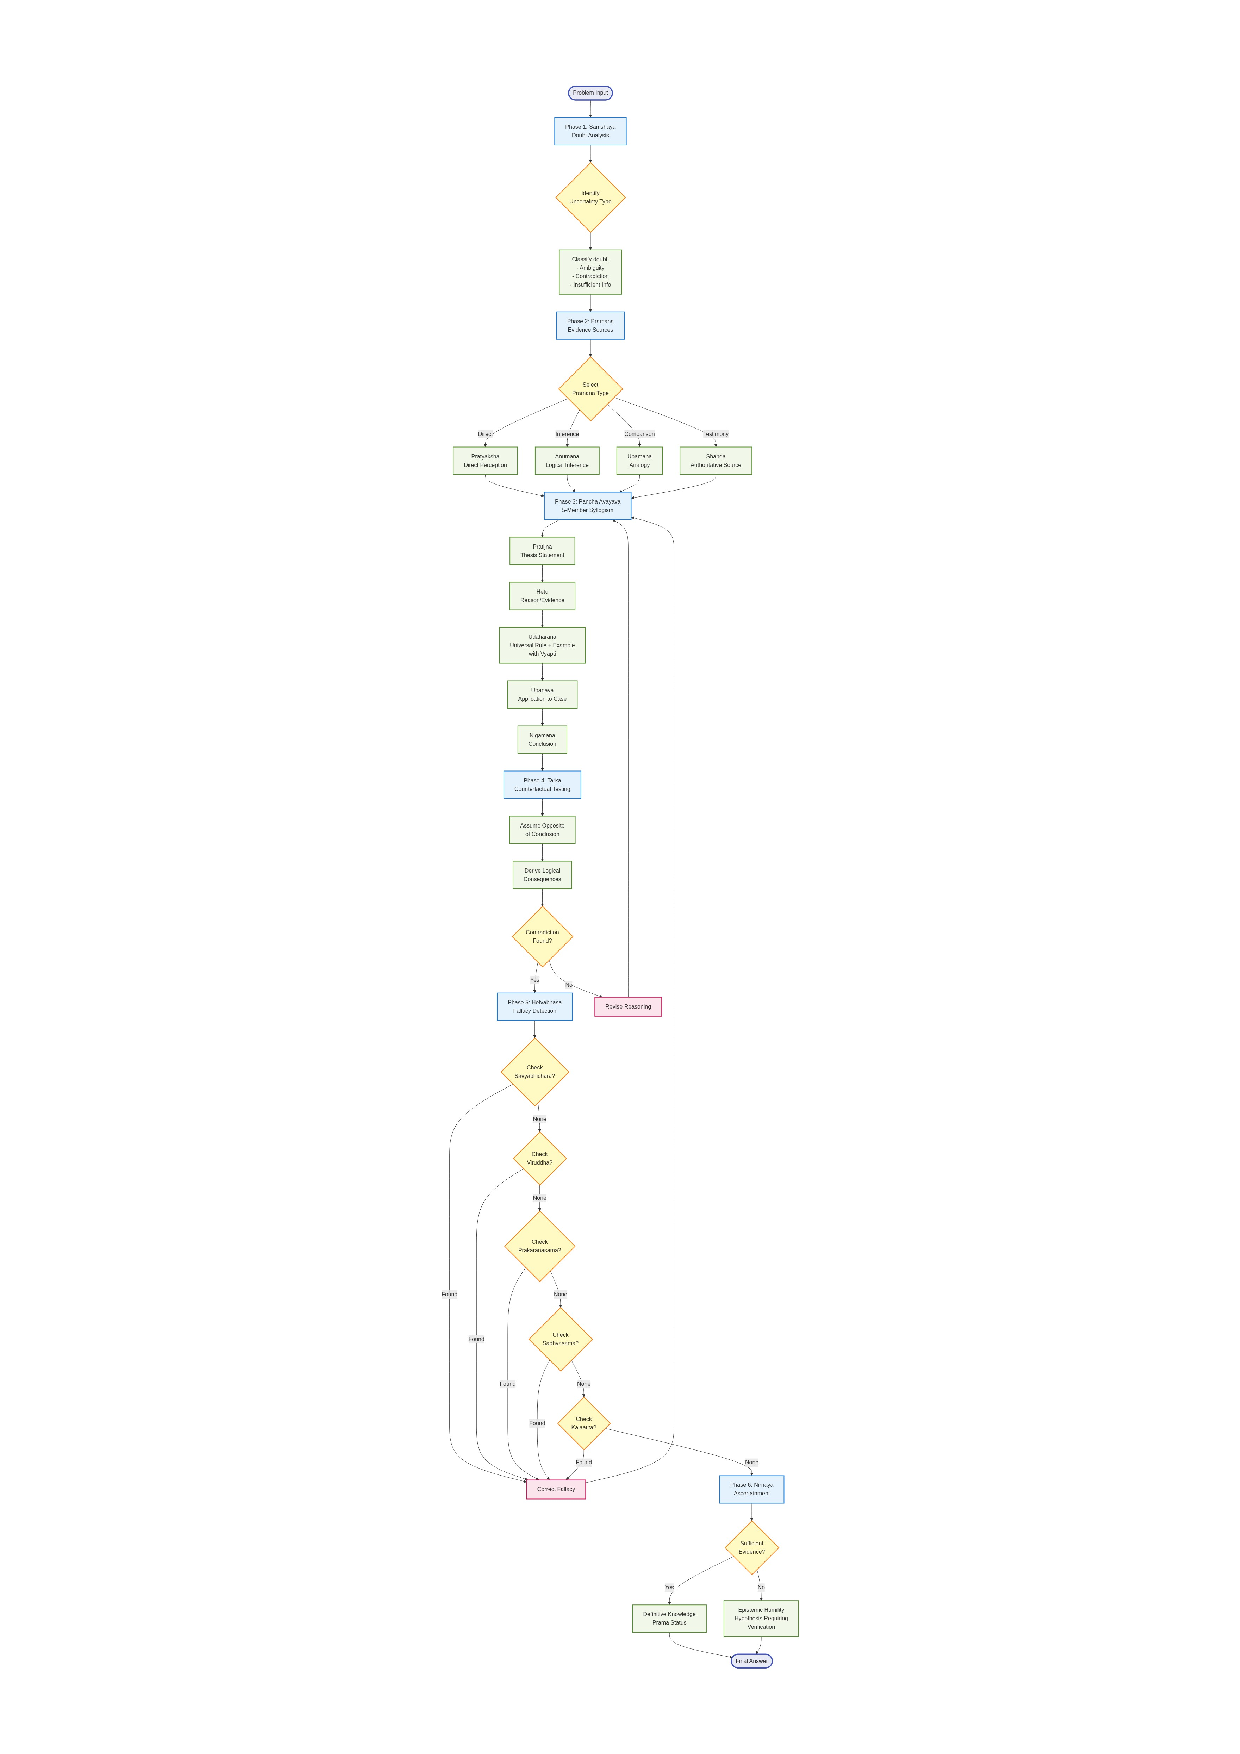
\includegraphics[width=0.9\textwidth]{figures/nyaya_flow.pdf}
\caption{The six-phase Nyaya reasoning flow: Samshaya (Doubt) $\rightarrow$ Pramana (Evidence) $\rightarrow$ Pancha Avayava (Syllogism) $\rightarrow$ Tarka (Counterfactual) $\rightarrow$ Hetvabhasa (Fallacy Check) $\rightarrow$ Nirnaya (Conclusion).}
\label{fig:nyaya_flow}
\end{figure}

\subsection{Theoretical Foundations}
\label{subsec:theoretical_foundations}

Our adaptation of Nyaya reasoning consists of six structured phases, each serving a specific epistemic function. Unlike generic chain-of-thought prompting, this framework enforces explicit epistemological structure that prevents the ``pattern-matching masquerading as reasoning'' problem identified in current LLMs~\cite{apple-gsm-symbolic-2024}. The complete reasoning flow is illustrated in Figure~\ref{fig:nyaya_flow}.

\subsubsection{\samshaya{} (Doubt Analysis)}

The first phase requires identifying and classifying the type of uncertainty or ambiguity in the problem. In Nyaya epistemology, inquiry only begins when there is genuine doubt---forcing the model to articulate what is uncertain prevents jumping to conclusions.

We recognize five categories of doubt:

\begin{enumerate}
    \item \textbf{Samana Dharma Upapatti}: Multiple entities share properties, creating ambiguity about which entity satisfies a given constraint. This is the most common type in constraint satisfaction problems.
    \item \textbf{Aneka Dharma Upapatti}: A single entity has multiple conflicting properties, requiring resolution of the contradiction.
    \item \textbf{Vipratipatti}: Contradictory testimony from multiple sources, requiring reconciliation.
    \item \textbf{Upalabdhi Avyavastha}: Uncertainty about the validity of perception or observation.
    \item \textbf{Anupalabdhi Avyavastha}: Uncertainty arising from the absence of expected evidence.
\end{enumerate}

\textbf{Computational requirement}: The model must explicitly identify which category applies and justify why this doubt is worthy of investigation. This prevents premature pattern-matching to likely answers.

\textbf{Example classification}: For a constraint satisfaction problem like ``Alice, Bob, and Carol each have a pet (cat, dog, fish). Alice doesn't have the cat. Bob has the dog,'' the doubt type would be \textit{Samana Dharma Upapatti} because multiple entities (Alice, Bob, Carol) share the property of ``having a pet,'' creating ambiguity about which entity has which pet.

\subsubsection{\pramana{} (Evidence Sources)}

The second phase identifies valid means of knowledge (\textit{pramāṇas}), preventing hallucination by forcing explicit grounding of all claims. Nyaya recognizes four types, all of which must be addressed:

\textbf{Pratyaksha (Direct Perception)}: Observable facts directly stated in the problem statement. The computational constraint is strict: \textit{only} verbatim or clear paraphrases from the input are allowed---no inferences. This can be validated programmatically via substring matching against the problem text. A common error is citing inferred facts as ``observed.''

\textbf{Anumana (Inference)}: Logical deductions with explicit inference type. We recognize three subtypes:
\begin{itemize}
    \item \textbf{Purvavat}: Cause $\rightarrow$ Effect (e.g., smoke implies fire)
    \item \textbf{Sheshavat}: Effect $\rightarrow$ Cause (e.g., flood implies prior rain)
    \item \textbf{Samanyatodrishta}: General correlation or transitive inference (e.g., if A > B and B > C, then A > C)
\end{itemize}

The constraint requires stating which inference type applies and showing the logical connection. A common error is treating correlation as causation (which maps to the \textit{Savyabhichara} fallacy).

\textbf{Upamana (Comparison)}: Knowledge through analogy to known solved cases. This enables case-based reasoning and few-shot learning. The constraint requires citing structural similarity to previous examples, not superficial metaphors. This is particularly useful for recognizing problem types (e.g., ``This is similar to the constraint satisfaction pattern seen in Problem X'').

\textbf{Shabda (Testimony)}: Authoritative logical principles or established rules. Examples include laws of logic (modus ponens, modus tollens), mathematical axioms, or universal principles. The constraint requires general principles, not problem-specific facts. A common error is restating the problem statement as a ``principle.''

\textbf{Mapping to formal logic}: In constraint satisfaction problems, \textit{Pratyaksha} corresponds to given constraints, \textit{Anumana} to logical deductions (transitive closure, elimination), \textit{Upamana} to recognizing problem structure, and \textit{Shabda} to universal logical rules (e.g., ``if X excludes Y and Y excludes Z, then X and Z are compatible'').

\subsubsection{\pancha{} Avayava (Five-Member Syllogism)}

The core deductive engine consists of five required components per inference step:

\begin{enumerate}
    \item \textbf{Pratijna (Thesis)}: The specific, testable claim being established (e.g., ``Bob has the dog'').
    \item \textbf{Hetu (Reason)}: Evidence supporting the claim, which must reference \pramana{} sources from Phase 2 (e.g., ``Because constraint 2 directly states this'').
    \item \textbf{Udaharana (Universal Example)}: \textit{Critical requirement}: Must contain both a universal rule (\textit{vyāpti}) in the form ``Wherever X, there is Y'' \textit{and} a concrete instance (\textit{dṛṣṭānta}). For example: ``Wherever a direct constraint assigns entity E to position P, there E occupies P. For instance, 'John sits in seat 5' means John is in seat 5.'' A common error is providing only a specific example without the universal rule.
    \item \textbf{Upanaya (Application)}: How the universal rule applies to the specific case at hand (e.g., ``This problem states 'Bob has a dog' as constraint 2'').
    \item \textbf{Nigamana (Conclusion)}: Restated thesis, now justified (e.g., ``Therefore, Bob has the dog'').
\end{enumerate}

\textbf{Comparison to Western syllogisms}: Unlike Aristotelian syllogisms (major premise, minor premise, conclusion), Pancha Avayava requires explicit universal rules with concrete examples (\textit{dṛṣṭānta}), preventing purely abstract reasoning disconnected from empirical grounding. This addresses a key failure mode in LLM reasoning where abstract patterns are applied without concrete validation.

\textbf{Multiple syllogisms}: Complex problems require multiple Avayava chains, each establishing a different intermediate conclusion that builds toward the final answer.

\subsubsection{\tarka{} (Counterfactual Testing)}

This phase verifies conclusions via reductio ad absurdum, serving as the self-verification mechanism that distinguishes genuine reasoning from lucky guesses.

\textbf{Requirements}:
\begin{enumerate}
    \item Assume the opposite of the conclusion
    \item Derive a logical contradiction or absurdity
    \item Demonstrate why the negation is impossible
    \item \textit{Not} just ``if X then X'' tautology---must test meaningfully
\end{enumerate}

\textbf{Feedback loop}: If Tarka reveals a contradiction, the model must return to earlier phases (particularly Pancha Avayava) to correct the reasoning chain. This creates a self-correcting mechanism.

\textbf{Example}: If the conclusion is ``Alice has the cat,'' the Tarka test would assume ``Alice does not have the cat.'' If this leads to a contradiction (e.g., ``But then no one has the cat, which violates the constraint that all pets are assigned''), the original conclusion is validated.

\subsubsection{\hetvabhasa{} (Fallacy Detection)}

This phase performs explicit self-audit for reasoning errors, preventing the model from accepting flawed arguments that ``look good'' syntactically. All five fallacy types must be checked:

\begin{enumerate}
    \item \textbf{Savyabhichara (Erratic Reason)}: The reason correlates with the conclusion but doesn't cause it. Example: ``The ground is wet, therefore it rained'' (could be a sprinkler). Maps to correlation vs. causation errors.
    \item \textbf{Viruddha (Contradictory Reason)}: The reason actually proves the opposite of the conclusion. Example: ``All ice is cold, this is ice, therefore it's hot.'' Maps to logical contradictions.
    \item \textbf{Prakaranasama (Irrelevant Reason)}: Circular reasoning or off-topic arguments. Example: ``X is true because X is true.'' Maps to begging the question, circular logic.
    \item \textbf{Sadhyasama (Unproved Reason)}: The premise needs as much proof as the conclusion. Example: ``Ghosts exist because I saw a ghost.'' Maps to assuming what needs to be proved.
    \item \textbf{Kalaatita (Mistimed Reason)}: Reasoning depends on invalid temporal assumptions. Example: Using outdated information as if current. Maps to temporal logical errors.
\end{enumerate}

\textbf{Systematic error checking}: Each fallacy type is checked explicitly, and if detected, the model must correct the reasoning in earlier phases.

\subsubsection{\nirnaya{} (Ascertainment)}

The final phase reaches a definitive conclusion \textit{or} explicitly states that insufficient evidence exists for certainty. This enforces epistemic humility---the model must distinguish knowledge from hypothesis.

\textbf{Two valid outcomes}:

\begin{enumerate}
    \item \textbf{Definitive Knowledge (Prama)}: The conclusion survived all tests (Tarka, Hetvabhasa), answer provided with confidence, status marked as ``Definitive Knowledge.''
    \item \textbf{Epistemic Humility}: Insufficient \pramana{} sources to reach certainty, explicitly stating what additional evidence is needed, status marked as ``Hypothesis Requiring Verification.''
\end{enumerate}

\textbf{Preventing hallucinated confidence}: By requiring explicit acknowledgment of uncertainty when evidence is insufficient, Nirnaya prevents the common LLM failure mode of confidently asserting answers without proper justification.

\subsection{Computational Requirements}
\label{subsec:computational_requirements}

The Nyaya framework imposes specific computational requirements that differ from standard chain-of-thought prompting.

\subsubsection{Token Budget Analysis}

For a typical 4-variable constraint satisfaction problem, we estimate token requirements by phase:

\begin{itemize}
    \item \samshaya{}: 50--100 tokens (doubt classification + justification)
    \item \pramana{}: 200--400 tokens (4 sources $\times$ evidence + structured format)
    \item \pancha{} Avayava: 300--600 tokens (3--5 syllogisms $\times$ 120 tokens each)
    \item \tarka{}: 100--200 tokens (counterfactual test + contradiction derivation)
    \item \hetvabhasa{}: 150--250 tokens (5 fallacy checks + reasoning)
    \item \nirnaya{}: 50--100 tokens (conclusion + justification)
\end{itemize}

\textbf{Total}: 850--1,650 tokens (median: $\sim$1,250 tokens).

\textbf{Comparison baseline}:
\begin{itemize}
    \item GPT-4 standard CoT: 200--400 tokens for the same problem
    \item o1-preview (internal reasoning): 500--800 tokens
    \item Pramana Nyaya: 1,250 tokens (fully explicated structure)
\end{itemize}

\textbf{Overhead ratio}: 3--6$\times$ vs. standard CoT.

\textbf{Justification}: The overhead buys \textit{interpretability} and \textit{audit trail}. Similar to formal mathematical proof vs. informal argument---longer but verifiable. Each phase serves an epistemic function:
\begin{itemize}
    \item Prevents conflation of evidence types (\pramana{} separation)
    \item Forces explicit universal rules (Udaharana ``Wherever X'')
    \item Enables error detection (\tarka{} + \hetvabhasa{})
    \item Distinguishes knowledge from hypothesis (\nirnaya{})
\end{itemize}

For high-stakes reasoning (medical diagnosis, legal arguments, safety-critical systems), 3--6$\times$ overhead is an acceptable tradeoff for trustworthiness.

\subsubsection{Phase Quality Dependencies}

The phases form a critical path: \pramana{} $\rightarrow$ \pancha{} Avayava $\rightarrow$ \nirnaya{}. 

\textbf{Dependency chain}:
\begin{itemize}
    \item Weak \pramana{} $\rightarrow$ Invalid Hetu in Avayava $\rightarrow$ Wrong conclusion
    \item Missing \tarka{} $\rightarrow$ Can't catch errors in reasoning chain
    \item Incomplete \hetvabhasa{} $\rightarrow$ Fallacies slip through undetected
    \item Poor Udaharana (no universal rule) $\rightarrow$ Argument not generalizable
\end{itemize}

\textbf{Phase quality thresholds} (for overall solution validity):

\begin{table}[h]
\centering
\small
\begin{tabular}{lcc}
\toprule
Phase & Minimum Requirement & Score if Failed \\
\midrule
\pramana{} & All 4 types present with content & 0/10 if any missing \\
\pancha{} Avayava & $\geq$2 complete syllogisms with universal rules & 0/10 if $<$2 valid \\
\tarka{} & Must test conclusion (not tautological) & 0/10 if circular \\
\hetvabhasa{} & All 5 fallacy types checked & Partial credit if $\geq$3 \\
\samshaya{} \& \nirnaya{} & Structural presence & Pass if present \\
\bottomrule
\end{tabular}
\caption{Phase quality thresholds for solution validity. A solution can have all 6 phases present but still score poorly if phases are empty template-filling. Quality $>$ format compliance.}
\label{tab:phase_quality}
\end{table}

\subsection{Data Format Specification}
\label{subsec:data_format}

\subsubsection{Format Selection Rationale}

We chose \textbf{structured Markdown with YAML frontmatter} for training examples:

\textbf{Advantages}:
\begin{itemize}
    \item Human-readable for manual creation (critical for Stage 0--1 seed examples)
    \item Machine-parseable for validation and training (via \texttt{MarkdownParser})
    \item Git-friendly for version control and collaboration
    \item Balances structure (YAML metadata) with natural flow (markdown prose)
    \item Easier to create than pure JSON (no quote escaping, better formatting)
\end{itemize}

\textbf{Rejected alternatives}:
\begin{itemize}
    \item Pure JSON: Too mechanical, hard to write manually
    \item Custom DSL: Adds complexity without clear benefit
    \item Unstructured text: Can't validate programmatically
\end{itemize}

\subsubsection{File Structure Template}

Every training example follows this structure (implemented in \texttt{src/pramana/application/data/parser.py}):

\begin{verbatim}
---
# YAML Frontmatter: Machine-readable metadata
id: pramana-[stage]-[number]
problem_type: constraint_satisfaction | boolean_sat | multi_step_deduction
difficulty: simple | moderate | complex
variables: [number]
ground_truth: "[Expected answer]"
metadata:
  created_date: YYYY-MM-DD
  author: manual | synthetic
  validated: true | false
  z3_verifiable: true | false
  stage: 0 | 1 | 2
---

# Problem

[Natural language problem statement]

**Constraints**:
1. [Constraint 1]
2. [Constraint 2]
...

**Question**: [What needs to be determined]

---

## Samshaya (Doubt Analysis)

**Doubt Type**: [One of 5 categories]
**Justification**: [Why this doubt exists]

---

## Pramana (Sources of Knowledge)

### Pratyaksha (Direct Perception)
- [Observable fact 1]
- [Observable fact 2]

### Anumana (Inference)
- [Inference with type]

### Upamana (Comparison)
- [Analogy reference]

### Shabda (Authoritative Principles)
- [Universal rule]

---

## Pancha Avayava (5-Member Syllogism)

### Syllogism 1: [Topic]
**Pratijna (Thesis)**: [Claim]
**Hetu (Reason)**: [Evidence]
**Udaharana (Universal + Example)**: Wherever [general rule], 
  there [consequence]. For example, [concrete instance].
**Upanaya (Application)**: [How rule applies here]
**Nigamana (Conclusion)**: Therefore, [thesis restated]

[Repeat for additional syllogisms]

---

## Tarka (Counterfactual Testing)

**Test**: Assume [opposite of conclusion].
[Derivation of contradiction]
Therefore, [original conclusion must be true].

---

## Hetvabhasa (Fallacy Detection)

Check for Savyabhichara: [none_detected | description]
Check for Viruddha: [none_detected | description]
Check for Prakaranasama: [none_detected | description]
Check for Sadhyasama: [none_detected | description]
Check for Kalaatita: [none_detected | description]

**Reasoning**: [Why no fallacies detected OR corrections made]

---

## Nirnaya (Ascertainment)

**Status**: Definitive Knowledge | Hypothesis Requiring Verification
**Answer**: [Final answer if definitive]
**Justification**: [Why certain OR what evidence missing]
**Confidence**: [High/Medium/Low with explanation]
\end{verbatim}

\subsubsection{Validation Schema}

Programmatic validation (implemented in \texttt{src/pramana/domain/validators/structure.py}) checks:

\begin{itemize}
    \item \textbf{Required sections}: All 6 phases present and in correct order
    \item \textbf{Pramana completeness}: All 4 types (Pratyaksha, Anumana, Upamana, Shabda) present
    \item \textbf{Pancha Avayava completeness}: $\geq$1 syllogism with all 5 members (Pratijna, Hetu, Udaharana, Upanaya, Nigamana)
    \item \textbf{Udaharana universal rule}: Must contain ``Wherever X, there is Y'' structure
    \item \textbf{Hetvabhasa completeness}: All 5 fallacy types checked
    \item \textbf{YAML frontmatter}: Required fields (id, problem\_type, ground\_truth) present
\end{itemize}

This validation ensures training examples meet structural requirements before model training, preventing format errors from propagating into learned behavior.
